% ========== VASKEBJØRN ==========
\begin{frame}{%
  \begin{minipage}[c]{0.30\textwidth}
    Vaskebjørn
  \end{minipage}%
  \hfill
  \begin{minipage}[c]{0.45\textwidth}
    \footnotesize
    \textbf{Jagttid:} Hele året\\
    \textbf{Regulering:} Uden aftale (invasiv)
  \end{minipage}%
  \hfill
  \begin{minipage}[c]{0.15\textwidth}
    \noindent\raggedleft
    
\includegraphics[width=0.5cm, height=0.5cm, keepaspectratio]{Billeder/Ikoner/star.png}
  \end{minipage}%
}
  \vspace{0.25em}
  \begin{columns}[T]
    % --- Venstre kolonne: Tekst ---
    \column{0.45\textwidth}
    \setlength{\parskip}{0.4em}
    \tiny
    \RaggedRight
    \textbf{\textit{Procyon lotor}} – invasiv art med karakteristisk ansigtsmaske og stribet hale. \par
    \textbf{Udseende:}\\
    \quad – Grå pels med lange sorte og hvide dækhår \\
    \quad – Hale halvt så lang som kroppen og stribet \\
    \quad – Sort tværstribet ansigtsmaske
    % --- Højre kolonne: Større billede ---
    \column{0.52\textwidth}
    \centering
    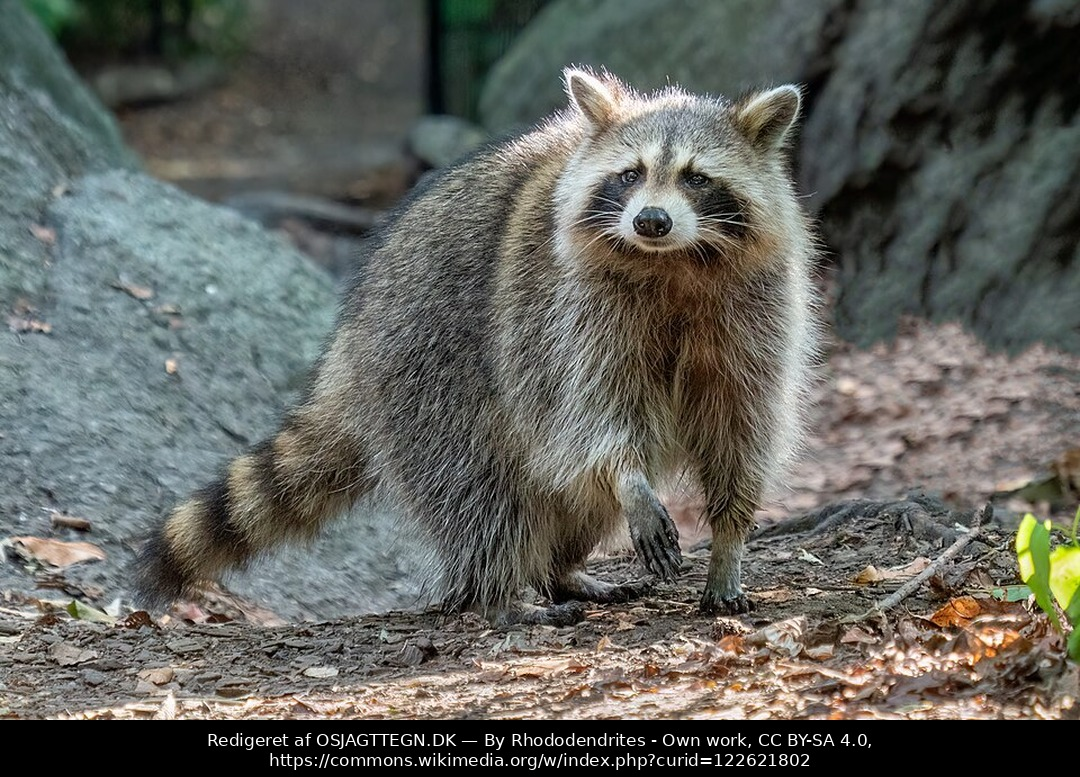
\includegraphics[width=\linewidth, height=7.2cm, keepaspectratio]{Billeder/Dyr/Pattedyr/rovdyr/vaskebjørn/vaskebjoern-01.jpg}
  \end{columns}
\end{frame}